\chapter{Literature Survey and Review}

\section{Coordination}

\paragraph*{}
Swarm robotics solution is a design architecture that obtains inspirations from biological interactions; thus, they should operate autonomously to solve problems rather than relying on a central authority\cite{turkler2022usage}. This decentralised approach is also crucial to achieve increased resilience and flexibility given a complex environment of deployment\cite{das2024bio}.

\paragraph*{}
Communication protocols can be categorised into two principal types depending on the nature of information transmission: Direct communication and Indirect communication\cite{das2024bio}. Direct communication refers to robotic agents that are able to coordinate via networked communication. Direct communication use cases are highlighted in many studies.

\paragraph*{}
Ibrahim et al. \cite{ibrahim2024enhancing} studied direct communication to determine the optimal distance for robotic agents to achieve consensus. Three strategies were tested within a 50 cm range: Close-neighbour, Far-neighbour, and Rand-neighbour. Close-neighbour excels in stable environments but performs poorly in complex ones. Both Close-neighbour and Far-neighbour introduce bias, reducing accuracy. Rand-neighbour, which randomly selects swarm members for communication, proved superior due to efficient information flow and minimal bias. This strategy can be one of our key designs for swarm communication in this project.

\paragraph*{}
Ayari and Bouamama\cite{ayari2023evolutionary} and Perera et al.\cite{perera2022integrating}, S et al.\cite{sr2023control} and Z. Wang et al.\cite{wang2024decentralized} conducted studies to promote robots’ actions based on their sensory observations and objectives. S et al.\cite{sr2023control} proposed a Multi-Agent Deep Deterministic Policy Gradient (MA-DDPG), an observation-based decision making flow with an architectural twist, where there is a central swarm manager that evaluates decentralized agents' reinforcement learning for optimal rewards. Z. Wang et al.\cite{wang2024decentralized} proposed increasing sensory inputs from both visual data and communication for redundancy, which highly aligns with the proposed swarm system.

\paragraph*{}
Yasser et al.\cite{yasser2024optimized} expanded more on Clustered Dynamic Task Allocation (CDTA), an approach to dynamically assign tasks based on swarm state and the environment \cite{nedjah2021communication}, for the purpose of increasing the velocity of swarm communication. They proposed CDTA-CL (Centralized Loop) and CDTA-DL (Dual Loop). CDTA-CL sends information to the leader for computation, while CDTA-DL compares information before sending it to the leader. CDTA-DL outperformed CDTA-CL, increasing speed by 75.976\% compared to 54.4\%. CDTA-DL will be considered as a design pillar for this project.

\paragraph*{}
In addition to direct communication improvements, indirect communication, known as Stigmergy, also plays a significant role in swarm intelligence. This concept involves individual robot actions modifying the environment, impacting the decision-making of other robots. For example, construction robots can leave blocks and materials to signal ongoing work\cite{das2024bio}. This is an intriguing notion to consider in the interaction of the swarm system.

\paragraph*{}
For effective communication, especially in interdependent tasks, robots need to be aware of each other and task requirements. Semantic communication, where contextually relevant data is prioritized, is necessary\cite{beck2023swarm}. The balance between communication and context must align with task demands. High sensory data tasks require reliable, real-time communication, while tasks with lower communication demands can prioritize contextually relevant information\cite{zhang2021cooperative}.

\section{Object Detection}

\paragraph*{}
Object Detection plays a crucial role in computer vision by identifying and locating objects within images or video feeds. Its primary goal is to identify objects as well as determining its precise location through bounding boxes. In order for the robots to interact with the environment and eventually complete their task, it is crucial that they have to understand the dynamic and complex surroundings with their sensors, followed by recognising all targets around them as well as targeting them. Another key requirement is that each robot should distinguish other team members from objects in the environment, known as “Kin detection”, and know their relative position to others with data from their sensors

\paragraph*{}
In various real-world applications, such as autonomous vehicles \cite{redmon2016yolo} and multi-robot coordination in warehousing \cite{kumar2018multi}, 2D object detection is effective for basic identification and localization tasks. However, detecting objects in complex environments presents challenges, particularly when object occlusion occurs \cite{girshick2014rich}. The limitations of 2D object detection, which relies on single-plane images, make it difficult to accurately identify objects that are distant or situated in cluttered settings \cite{chen2023object}.

\paragraph*{}
Three-dimensional data can be acquired using various devices such as RADAR, RGB-D cameras, and stereo cameras \cite{karin2023comparative}. Each of these devices has distinct advantages and disadvantages:

\paragraph*{}
RADAR employs radio signals to measure distance and estimate the shape and size of objects but does not detect colour and has low spatial resolution \cite{karin2023comparative}. This limitation makes it challenging to distinguish between closely spaced or thin objects \cite{wang2020radar}. However, RADAR is particularly effective in poor visibility conditions, such as for collision avoidance and adaptive cruise control.

\paragraph*{}
RGB-D cameras, like the Intel RealSense D455, capture both colour and depth information, which allows for detailed spatial analysis \cite{tychola2022reconstruction}. These cameras use techniques such as time-of-flight and structured light to measure depth \cite{tychola2022reconstruction}. The data from RGB images and depth maps can be processed to create 3D point clouds or models, facilitating object detection and scene analysis. These cameras are adept at perceiving attributes like colour and shape in real-time, making them suitable for dynamic environments. Nonetheless, their performance can be impacted by lighting conditions, which affects depth accuracy, and they have a more limited sensing range compared to RADAR.

\paragraph*{}
Stereo cameras operate with two lenses, capturing left and right images to mimic human vision \cite{medathati2016bio}. The data collected typically consists of a 3D point cloud that shows the spatial distribution of objects in the environment. Creating this 3D point cloud involves processing stereo images to identify matching points and calculate their depth. While stereo cameras can detect distant and small objects due to their dense pseudo point cloud\cite{li2024object}, they may struggle with object detection in dynamic environments because of noise in the point cloud data during rapid changes\cite{eppenberger2020leveraging}.

\paragraph*{}
Considering stereo camera and RGB-D camera performance, as it can perceive colour which is the main characteristic that is required in object detection and classification, in 3D object detection. The RGB-D camera produces 0.82\% average percentage error, while the stereo camera produces 2.61\% average percentage error measuring under the same condition and doing the same tasks in multi-object detection\cite{rodriguez2021comparison}. 

\paragraph*{}
Considering the data format obtained from the selected device which is the RGB-D camera will help to identify the suitable candidate of the 3D object detection approach. The input RGB-D data contain two formats, one with normal colour image which is red,green, and blue, another one uses black and white to represent the distance information in a single channel, The darker colour represents an object that is further from the camera than the ones with lighter colour. 

\paragraph*{}
Given the variety of tools and algorithms used in 3D object detection research with RGB-D cameras, a proper quantitative comparison has not been consistently conducted. Only a few approaches can be categorised into one of the four main groups of 3D object detection. Therefore, this section aims to provide an overview of the key techniques used. Each technique will include a discussion of its core concepts, along with its strengths and weaknesses. A quantitative comparison will be presented at the end of this section.

\paragraph*{}
There are four major categories for 3D object detection using RGB-D cameras. Firstly, \textbf{2.5D processing methods}. This method utilises the 3D convolution kernel The concept of this method is to use depth images obtained from the RGB-D camera as 2D images directly. Additionally, HHA encoding is used for enhancing the geometric representation including object’s height, surface angle compared to the ground etc.\cite{wang2021recent}. The combination of RGB and depth data in this approach enhances detection accuracy, especially in complex environments\cite{wang2021recent}\cite{arican2017object}. However, it can potentially perform not so well in highly dynamic or unstructured scenes especially when depth data is less accurate\cite{wang2021recent}.

\paragraph*{}
Secondly, \textbf{2D Driven 3D Methods} combine 2D object detection techniques with 3D processing to increase efficiency of 3D object detection. It basically narrows down the space with 2D detection followed by refining and defining 3D object boundaries using depth data. While RGB data remain unchanged, the depth data are transformed into point clouds\cite{wang2021recent}.  A more advanced model called “ The series of Frustum PointNet” which utilises RGB-D data for enhanced 3D object detection by integrating 2D image information (RGB data) with 3D point cloud data. 3D fustrums are transformed from 2D object proposals using camera projection metrics allowing effective feature extraction and object localisation using several advanced neural networks e.g. PointNet and LDG CNN. The integration of RGB and depth data boost the detection performance especially in small object detection like pedestrian as well as optimise computational resources while maintaining high detection rates\cite{paigwar2021frustum}. However, the complexity of the system and processing time can be increased from relying on both point cloud and RGB data\cite{tao2023fpvnet}. 

\paragraph*{}
\textbf{Geometric Descriptor-based Methods} utilises depth information from RGB-D camera for enhancing object recognition capabilities by using geometric features extracted from RGB image and depth data. This category comprises three main methods; Centre of Gravity (COG) utilises the geometric centre of the detected objects’ features to improve the accuracy of the objects’ localisation. The boundaries of the object are refined and the detection reliability is enhanced by analysing spatial distribution of points in 3D space. Latent Surface Shape (LSS) identifies the pattern of the indoor settings by focusing on the surface that an object rests on. This approach helps explain the differences in object shapes. Although this approach allows small object detection to be done easier, it can struggle with objects with unclear supporting surfaces\cite{ren2018three}. Lastly, H3DNet\cite{zhang2020h3dnet} is a neural network that uses geometric shapes to detect objects. A detailed description of points is created for predicting the object's shapes. This is then used to make and improve proposals of object detections. The network refines object detection by adjusting the bounded box or other geometrical shape followed by classifying the object and eventually adding labels\cite{wang2021recent}.

\paragraph*{}
Lastly, \textbf{3D convolution based models} which highlight the importance of texture data that is obtained from the 3D object detection. There are several methods utilising both image and point clouds for enhancing overall performance with fusion schemes implementation. 

\paragraph*{}
The series of sliding windows including The Sliding Shapes method and Deep Sliding Shapes (DSS). The Sliding Shape approach performs the object classification using 3D sliding windows which are able to handle occlusions and changes in viewpoint effectively. However, the processing can be slowed down due to the hand-crafted features which this method relies on extensively. For the Deep Sliding Shapes, a 3d convolutional neural network (CNN) is used to improve the efficiency upon the Sliding Shapes method. This significantly solved two main challenges; speeding up the target detection and eliminating the need of CAD design that is done manually. Although the performance is enhanced, the demand for higher computation which is a result of 3D convolutions complexity. 

\paragraph*{}
VoteNet employs the voting mechanism when locating objects as well as generating high quality proposals which both help solve the sparse point cloud issue, but this can be limited by noisy or missing data points. Additionally, imVoteNet is built on the VoteNet by incorporating 2D image data together with texture and semantic information added. This enhances the object detection performance especially when there is a sparse point cloud data. Although the 2D and 3D data fusion increases the accuracy, the complexity is raised as well.

\paragraph*{}
The VoteNet's object detection is enhanced by BRNet which traces representative points back to their original vote centres and re-examining point clusters, allowing a more detailed understanding of object structures which also comes with higher cost of computational requirement due to higher complexity. MLCVNet improves VoteNet's performance by incorporating multi-level contextual information which enables the model to better grasp the relationships between objects and their surroundings, leading to more accurate detections. However, the increased complexity of simultaneously modelling both global and local context causes higher computational costs. 

\paragraph*{}
The Hierarchical Graph Network (HGNet) is the VoteNet method that adopts a graph-based approach for improving object detection performance. This features a shape-attentive feature extractor as well as integrated global scene contect, making the prediction even more accurate. However, the improved detection precision of this approach leads to higher computational cost as well.

\paragraph*{}
The author performs comparison of the 3D object detection performance of each approach by using the SUN RGB-D dataset which is a single-view RGB-D dataset containing 47 distinct indoor scenes shown in Figure 3.1. 

\begin{figure}
    \centering
    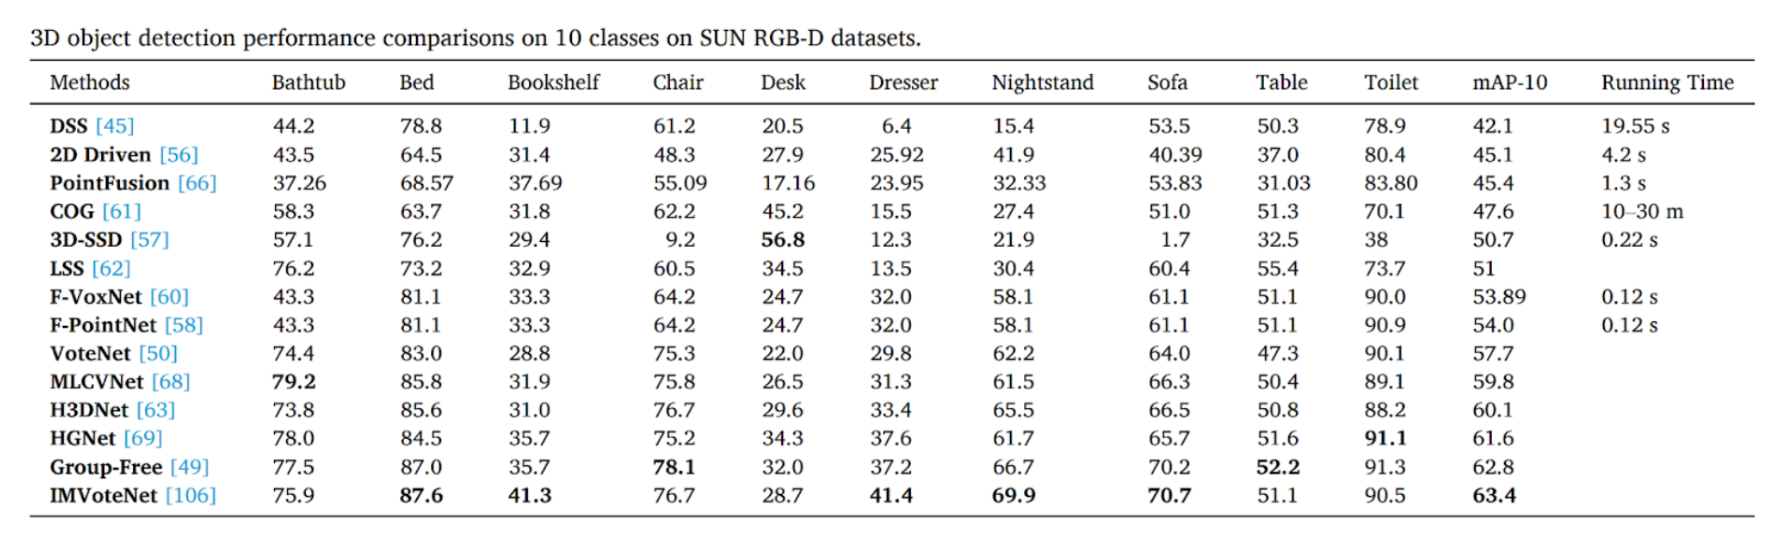
\includegraphics[width=0.8\linewidth]{assets/images/literature_survey/table_1.png}
    \caption{3D object detection performance comparisons on 10 classes on SUN RGB-D datasets. Table reused from \textit{Recent advances in 3D object detection based on RGB-D: A survey}\cite{wang2021recent}}
    \label{fig:3D object detection performance comparisons on 10 classes on SUN RGB-D datasets.} 
\end{figure}


\paragraph*{}
Although 3D convolution-based models tend to outperform other approaches, it's important to consider additional factors when selecting a method for our project, such as computational requirements, cost, deployment, integration with SLAM, and hardware compatibility.

\paragraph*{}
As some 3D object detection approaches build upon 2D object detection methods, such as convolutional networks, it’s equally important to evaluate the various available 2D object detection approaches in terms of their concepts, functionality, and performance.

\paragraph*{}
There are two major stages in 2D object detection development; the traditional stage and the new stage with deep learning. The concept of traditional object or target detection uses sliding window methods to generate boxed on target images or videos followed by manual feature extraction. Lastly, classifiers like Support Vector Machine (SVM)  and Logistic regression will classify the extracted features and there will be a box bounded around the target position. This can be seen in some models like SIFT and Cascades and some typical algorithms are HOG\cite{dalal2005histograms}, Viola Jones\cite{viola2001robust}, etc. which have limitations causing low detection speed and precision.

\paragraph*{}
In the second stage, Convolutional Neural Network (CNN) helps increase average detection accuracy by approximately 30\%\cite{zhou2023review}. There are two major algorithms in target detection with deep learning, one stage target detection and two-step target detection. 

\paragraph*{}
One-stage object detection algorithms predict both the coordinates and class probabilities of objects in a single step using a single neural network\cite{karbouj2024comparative}. Two prominent examples of these algorithms are Single Shot MultiBox Detector (SSD) and You Only Look Once (YOLO), both of which perform differently in various applications. SSD employs a VGG16 backbone for feature extraction and generates predictions at multiple layers, enabling it to handle objects of varying scales without the need for a region proposal network\cite{liu2016ssd}. On the other hand, YOLOv8, the latest iteration of the YOLO family, uses a more advanced Dark-53 backbone, alongside improved data augmentation techniques and anchor box clustering, which collectively boost its accuracy and efficiency\cite{zhou2023review}. To compare the performance of SSD and YOLOv8 in multi-object detection tasks, factors such as accuracy, adaptability, and speed are analysed. This comparison is based on the findings from the study "Performance Analysis of YOLOv8, RCNN, and SSD Object Detection Models for Precision Poultry Farming Management," where SSD, YOLOv8, and Faster R-CNN were tested for multi-object detection, as shown in Table 3.1. 

\paragraph*{}
Additionally, Two-stage Target Detection involves two steps: the first stage detects potential object locations, while the second stage refines these locations using a deep neural network to extract features from the proposed regions\cite{karbouj2024comparative}. The addition of a Region Proposal Network (RPN) in the second stage introduces extra computational demands, resulting in higher processing time and hardware requirements compared to one-stage detectors\cite{lin2017feature}. The main detectors in this category include;  R-CNN detector uses selective search to generate region proposals before applying CNN to each region to classify the target and bound each target with boxes. However, this approach is computationally  expensive as thousands of regions are processed by CNN independently\cite{girshick2014rich}.

\paragraph*{}
Fast R-CNN improves R-CNN by integrating region proposal generation and classification into one network for faster processing. It uses a CNN to process the image and classify ROIs from a shared feature map but still relies on external region proposals, limiting its real-time performance\cite{girshick2015fast}.

\paragraph*{}
Faster-CNN eliminates the need of selective search as it features an internal Regional Proposal Network (RPN) offering a strong balance between speed and accuracy which makes it suitable for real-time task\cite{ren2015faster}.
     
\paragraph*{}
In addition to the aforementioned characteristics of various one-stage and two-stage target detection algorithms, three selected models; YOLOv8, SSD, and Faster-CNN are compared focusing on their speed, precision, and adaptability. The result is measured from the multi-object detection in precision poultry farming management. 

\paragraph*{}

\begin{table}[!h]
\centering
\begin{tabular}{| p{3.5cm} | p{3cm} | p{4cm} | p{3.5cm} |}
    \hline
    Algorithms  & Recall Value  & Mean Average Precision (mAP@0.5)  & Precision \\ \hline
    YOLOv8  & 1.00  & 98.7\%  & 96.77\% \\ \hline
    SSD  & 0.65  & 77\%  & 89\% \\ \hline
    Faster R-CNN  & 0.67  & 59\%  & 77\% \\ \hline
\end{tabular}
\caption{A comparative analysis of YOLOv8, SSD, and Faster R-CNN based on key performance metrics, including Recall Value, Mean Average Precision (mAP@0.5), and Precision. Table reused from \textit{Performance analysis of YOLOv8, RCNN, and SSD object detection models for precision poultry farming management}\cite{kaliappan2023performance}}
\label{tab:performance_metrics}
\end{table}

Following this comparison, it is evident that YOLOv8 excels in multi-object detection, combining high accuracy with balanced speed and efficiency. This makes YOLOv8 particularly well-suited for real-time applications. Furthermore, YOLOv8’s lower hardware demands make it a more practical choice compared to the more resource-intensive Faster R-CNN and other two-stage detectors\cite{kaliappan2023real}.

\section{SLAM}

\paragraph*{}
SLAM, or Simultaneous Localization and Mapping, is a widely spread algorithm for navigation in the field of mobile robotics because of the exponential improvement in computer processing speed and the accessibility of sensors such as cameras and LiDAR \cite{barbadekar2023exploring}. Using SLAM, a mobile robot can construct an internal environment map while simultaneously using the map to estimate its location without needing predefined knowledge of area \cite{durrant2006simultaneous}.

\paragraph*{}
Environment mapping is one of the vital techniques in SLAM. The algorithm consists of building a mathematical model for the spatial information of an actual environment, which encapsulates the necessary information for navigation and interaction. However, as for the SLAM technique, additional requirements are needed; the mathematical model must be able to represent the robot’s state and the position of landmarks relative to the robot’s location \cite{durrant2006simultaneous}. Hence, the challenge with the requirements is that the robot must perform the localization and the mapping simultaneously.

\paragraph*{}
Given these complexities, the backbone of all principal SLAM methods is the utilization of these SLAM frameworks consisting of odometry, landmark prediction, landmark prediction, landmark extraction, data association, and matching, pose estimation, and map update \cite{chong2015sensor}.

\paragraph*{}
Building on this, situational awareness becomes an extreme component of SLAM, the precision and accuracy of the robot's perception play a huge role in defining the characteristics of other variations of the SLAM implementation. Therefore, a thorough understanding of advantages and disadvantages of each common perception device is an imperative concept not just for the robot’s components but also the structure of the SLAM’s backend algorithm. 

\paragraph*{}
Firstly, acoustic sensors are widely used across the preliminary stage of SLAM implementations to minimize the pose drift with time, with most of the sensors being SONAR, or Sound Navigation and Ranging \cite{udugama2023evolution}. These sensors are well operated in dark environments, as well as dusty and humid, due to their insensitivity towards illumination and opaqueness \cite{sahoo2019advancements}. 

\paragraph*{}
Secondly, LiDAR, or Light Detection and Ranging Sensor, is relatively similar to an ultrasonic sensor in terms of functionality \cite{udugama2023evolution}. However, LiDAR uses electromagnetic waves as a radiation reference instead of acoustic waves. A LiDAR renders a 3-dimensional representation of its surroundings known as the Point Cloud \cite{bisheng2017progress}. The strength of LiDAR is that the sensor can provide 360 degrees of perception with high precision \cite{cadena2016past}.

\paragraph*{}
Thirdly, depth cameras' mechanism works based on the illumination of the site with infrared light and measures the time-of-flight \cite{langmann2012depth}. Comparing the range of measurement and accuracy, a depth camera performs poorer than a 3D LiDAR scanner because the depth camera can only acquire data within a limited range of field of view; moreover, environmental factors may affect the accuracy of the depth camera; for example, the depth camera’s output is susceptible to certain materials of surfaces, such as reflective or transparent materials \cite{peng2023depth}. However, a depth camera is still a popular option for SLAM as it's a relatively economical device compared to its relatives, 3-D LiDAR, for instance.

\paragraph*{}
Ultimately, event-based cameras present the local bitmap-level motion alterations to an event that took place, which is different from conventional framing-based cameras \cite{udugama2023evolution}. The new technique has gained popularity more recently in the field of SLAM as an event-based camera yields more efficient computational performance and better overall accuracy \cite{huang2023event}.

\paragraph*{}
After reviewing the different sensors and addressing technological advancements available in today’s world, it is crucial to understand how researchers have implemented those ideas to different variations of SLAM. This understanding helps in overcoming challenges and limitations that their predecessors had faced and set new standards for new research frontiers. Moreover, it becomes essential to effectively classify those SLAM variations under different criteria.

\paragraph*{}
Li et al.\cite{li2024object} perfectly encapsulated how SLAM techniques can be classified: 

\paragraph*{}
Simultaneous Localization and Mapping (SLAM) techniques can be categorized by using different factors. Firstly, they can be divided into categories based on the type of sensors employed. They may include vision-based SLAM using cameras, LIDAR-based SLAM using LIDAR sensors, and RGB-D SLAM, which combines RGB cameras with depth sensors. Secondly, feature-based SLAM, which tracks distinguishing characteristics and direct SLAM, which executes mapping intensity or depth directly can be considered as different categories. Thirdly, the estimated approach, such as filter-based SLAM, which uses filters such as Particle Filter and graph-based SLAM, which is formulated as a graph optimization problem, provides another classification criterion. Finally, SLAM can be categorized based on time synchronization, with offline SLAM processing data in batches after collection and online SLAM estimating pose and map incrementally in real-time.

\paragraph*{}
Among the various SLAM methods, one of the most well-known is Visual Slam, or V-SLAM, a variation of SLAM that uses images from cameras, ranging from a conventional camera to an RBD-D camera (depth and ToF camera). V-SLAM itself can be divided into two sub-categories \cite{benkis2024survey}. Firstly, a feature-based SLAM system that matches camera data using sparse methods; one example of this robust and popular algorithm is the ORB-SLAM \cite{mur2015orb}. Secondly, the direct dense methods that evaluate based on the general luminance of the pixels in images, one of the famous algorithms is Direct Sparse Odometry \cite{engel2018direct}.

\paragraph*{}
In addition to V-SLAM, another key variation is LiDAR-based SLAM, which utilizes LiDAR sensors to localize itself by collecting data from its surroundings while building the map of the data representation. Registration algorithms, for instance, iterative closest point (ICP), are used to estimate the relative transformation of the point clouds during the operation \cite{gu2020review}. On the other hand, feature-based algorithms, such as LiDAR Odometry and Mapping, are used to represent 2D or 3D point cloud maps as grid maps \cite{zhang2014loam}. 

\paragraph*{}
Furthermore, by combining the strengths of different sensors and overcoming each’s limitations, the multi-sensor SLAM utilizes multiple sensors, such as cameras, Inertial Measurement Units (IMUs), Global Positioning System, LiDAR, etc. FAST-LIO, or a Fast LiDAR-Inertial Odometry, is a decent example of an algorithm that combines LiDAR feature points with IMU data \cite{xu2021fast}.

\paragraph*{}
As SLAM continues to evolve, one of the emerging trends is collaborative SLAM, especially in a distributed framework. This includes multi-robot SLAM that leverages stability of the system by minimizing global error accumulation, risk concentration \cite{chen2023overview}. 

\paragraph*{}
In this context, Slide-SLAM presents a real-time decentralized metric-semantic SLAM method that creates an object-based representation to append autonomous exploration functionality to a robot team. This is achieved by attaching a communication module to each robot, and then a unified map is obtained from each robot’s observation \cite{liu2024slideslam}.

\paragraph*{}
Similarly, C-SLAM, an open-source system of Swarm-SLAM that has main purposes to be a scalable, decentralized, and sparse system for multi-robot, especially swarm-like robot teams, to perform navigation operations in unknown environments. C-SLAM is designed to support IMU, LiDAR, stereo, and RGB-D sensing \cite{lajoie2024swarm}.

\section{Collective Movement}

\paragraph*{}
In the domain of swarm robotics, collective movement coordination and dynamic role assignment are crucial for enabling robots to work together efficiently. Research on coordinated motion in swarms often emphasises the need for algorithms that allow robots to adapt their roles and behaviours in real-time. For example, the study on "Efficient Strategies for Coordinated Motion and Tracking in Swarm Robotics" is a comprehensive overview of various coordination algorithms, contrasting different techniques for multi-robot collaboration. 

\paragraph*{}
The first coordination algorithm mentioned is the leader-follower model. This algorithm is rather straightforward in the sense that one or more robots are designated to guide the swarm while the other robots adjust their positions. The leader can be pre-programmed or autonomously chosen depending on the path while the followers maintain a set distance and set angle. This model as mentioned before is simple to apply while also being centralised providing clear direction for the followers. Additionally, the followers do not need the full knowledge of the environment meaning that this model can be scalable. However, this swarm being centralised means that it is prone to a single point of failure and having reduced flexibility \cite{mehta2024robust}. This model would only work well for a simple structured environment with predefined paths which unfortunately does not match with our objectives.

\paragraph*{}
Another coordination algorithm is the potential fields algorithm. This algorithm is based on virtual forces with each robot in the swarm being treated as a particle that is influenced by virtual forces exerted by other robots, obstacles and targets. These forces can attract or repel each other. The object is for the robot to be “pulled” towards the goal while avoiding collisions. This model has a couple advantages; namely: Decentralised control as each robot moves autonomously based on the forces acting on it, and smooth movements. However a couple of challenges come with it as well. One challenge is the possibility of the robot being stuck in a local minimum where virtual forces cancel each other out. Secondly, proper fine tuning of the force parameters is required to prevent the robot from oscillating \cite{martinez2023swarm}. Overall this approach could be useful for environments with many obstacles where smooth and continuous navigation can be important.  The third algorithm offered is the virtual force algorithm which is similar to the potential fields algorithm but with more constraints thereby being ineffectual to our project \cite{udugama2023evolution}. 

\paragraph*{}
When comparing these three algorithms above, potential field algorithm and virtual force algorithm are decentralised while the leader-follower model is centralised. While the leader-follower model offers a simple, scalable nature, it introduces a single point of failure. In contrast, the potential fields algorithm offers a more decentralised approach, which is better suited for dynamic environments but requires careful turning to avoid local minima.

\paragraph*{}
In swarm robotics, dynamic role assignment plays a crucial role in enabling robots to adapt their behaviours and tasks in real-time. One common method is insect-inspired behaviour, which mimics the role distribution seen in social insect colonies \cite{bonabeau1997adaptive}. In this approach, robots assume roles based on simple, local rules, such as task demand or proximity to a target, without centralised control. This method offers high scalability and robustness, as robots can seamlessly take on different tasks as needed, making it suitable for large swarms. However, its reliance on local information can sometimes lead to suboptimal task assignments, particularly in complex environments where global awareness might be needed.

\paragraph*{}
On the other hand, market-based approaches \cite{brambilla2012property} use a more structured mechanism where robots bid for tasks based on their capabilities and availability. This ensures that tasks are allocated to the most suitable robots, leading to more efficient task execution. However, the bidding process requires communication between robots, which may introduce delays and increase system complexity. While market-based approaches tend to be more optimal for task allocation, they may not scale as easily as insect-inspired methods, especially in large or dynamic environments where constant communication is challenging.

\paragraph*{}
Decentralised control in swarm robotics offers several key advantages, particularly in terms of scalability, robustness, and adaptability \cite{st-onge2023swarm}. In decentralised systems, each robot operates autonomously, relying on local information and interactions with neighbouring robots, which eliminates the need for a central controller. This allows the swarm to scale more easily, as adding more robots does not increase the computational or communication burden on a single entity. Additionally, decentralised systems are more robust, as the failure of one or more robots does not compromise the entire system; each robot can continue functioning independently. This is particularly advantageous in dynamic or unpredictable environments, where flexibility and fault tolerance are critical.

\paragraph*{}
In contrast, centralised control systems rely on a single controller to manage all robots, which creates a bottleneck as the number of robots increases. Centralised systems can suffer from single points of failure—if the controller fails, the entire system may halt. Moreover, communication delays and computational limits can hinder real-time performance in larger systems. While centralised control offers more efficient coordination in smaller, simpler environments, decentralised control is better suited for real-world applications where scalability and resilience are essential for handling complex and dynamic tasks.

\paragraph*{}
Despite significant advancements in swarm robotics and coordination algorithms, there remain notable gaps in applying these methods to practical, real-world environments such as cleaning tasks. Most research on algorithms like potential fields, leader-follower models, and market-based role assignment has focused on simulations or controlled environments, which often lack the complexity and unpredictability found in real-world scenarios. For instance, limited work has been done on integrating these algorithms with sensor-rich, dynamic settings where robots must navigate cluttered spaces, identify and manipulate diverse objects, and coordinate in real-time without centralised control. Additionally, the scalability of these systems is often not tested in practical, large-scale environments, such as a commercial building cleaning system, where communication constraints, battery life, and real-time decision-making are crucial factors.

\paragraph*{}